\documentclass[utf8x, 12pt]{G7-32} 


% --------- -------- SETTINGS --------- --------

% --------- Настройки стиля ГОСТ 7-32 --------

% Гипертекстовое оглавление в PDF
\usepackage[
bookmarks=true, colorlinks=true, unicode=true,
urlcolor=black,linkcolor=black, anchorcolor=black,
citecolor=black, menucolor=black, filecolor=black,
]{hyperref}

\usepackage{graphicx}   % Пакет для включения рисунков
\DeclareGraphicsExtensions{.jpg,.pdf,.png}
\geometry{right=20mm}
\geometry{left=30mm}
\usepackage{enumerate}
\setcounter{tocdepth}{3} % Подробность оглавления


% --------- other settings --------
\usepackage{MnSymbol}
%\usepackage{simpsons}
% --------- -------- SETTINGS --------- --------



\begin{document}

\frontmatter 

% --------- -------- TITLE --------- --------

\begin{center} 

\large САНКТ-ПЕТЕРБУРГСИЙ ГОСУДАРСТВЕННЫЙ ПОЛИТЕХНИЧЕСКИЙ УНИВЕРСИТЕТ

\large Кафедра Компьютерных Систем и Программных Технологий \\[5.5cm] 

\huge ОТЧЕТ \\[0.6cm] % название работы, затем отступ 0,6см
\large по лабораторной работе №1\\
\large Тема: <<Система вёрстки \TeX и расширения \LaTeX>>\\
\large Дисциплина: <<Методы и средства защиты информации>>\\[3.7cm]

\end{center} 

\begin{flushright}
Выполнил: студент гр. 53501/2 \\
Пономарев М.A. \\[1.2cm]


Преподаватель \\
Вылегжанина К.Д.
\end{flushright}


\vfill 

\begin{center} 
\large Санкт-Петербург \\
2015
\end{center} 

\thispagestyle{empty}


% --------- -------- TITLE --------- --------

\thispagestyle{empty}
\setcounter{page}{0}
\tableofcontents
\clearpage
\mainmatter



\chapter{Опыт работы}

На протяжении уже полугода я активно пользуюсь \TeX 'ом, за это время было два основных направления, где я применял эту систему вёрстки:

\begin{itemize}
	\item Подготовка студенческих отчётов
	\item Написание песенника для студенческого отряда Со$\largestar$
\end{itemize}


\section{Подготовка студенческих отчётов}

Как известно, у \TeX 'a есть несколько основных базовых классов. Функциональности, предоставленных ими вполне достаточно, чтобы написать простой студенческий отчёт. Захотелось писать их <<по--красивому>>, а именно найти в интернете специальный пакет или стилевой файл для написания отчётов по ГОСТу. 

Пришлось потратить много времени на поиски, в результате решил остановиться на стилевом пакете G7-32 --- в его названии кроется стандарт для написания студенческих отчётов, пояснительных записок, бакалаврских и магистерских работ. Данный отчёт написан, как раз с помощью этого пакета.

\section{Написание песенника для студенческого отряда}

Однажды была необходимость написать песенник для студенческого педагогического отряда, решил воспользоваться возможностями \LaTeX 'a. Трудность была в написании табулатуры к некоторым песням и схемы аккордов.

\begin{figure}[h]
	\begin{center}
		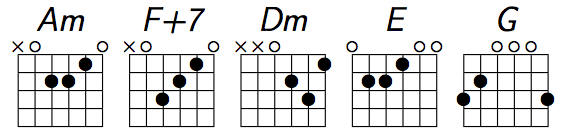
\includegraphics[width=7.0cm]{img/akk}
		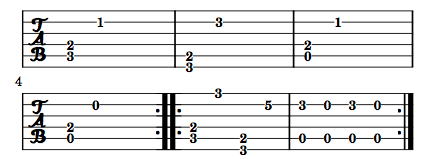
\includegraphics[width=7.0cm]{img/tab}
	\end{center}
	\vspace{-5mm}\caption{Схема аккордов (слева), табулатура (справа)}
\end{figure}	

Для написания аккордов был использован <<The Songs package>>, для табулатуры --- lilypond --- свободный нотный редактор. Поскольку он основан на \TeX 'е, то средствами этой среды есть возможность вставлять нотное описание прямо в документ, компилятор его проанализирует, создаст картинку и вставит в документ. На протяжении написания песенника возникало много разных сложностей, но в ходе их решения я узнавал много нового об этой системе вёрстки.

\chapter{Положительные впечатления}

Положительных моментов от пользования данной системы вёрстки очень много, опишу по пунктам некоторые из них:

\begin{enumerate}
	\item {\it Не волнуешься об отображении текста} Не надо волноваться о том, как написанный текст будет выглядеть, при использовании определенного класса заранее прописываются все настройки по вёрстке, тебе остается только наполнять документ контентом.
	\item {\it Text only} --- документ \TeX 'a является обычным текстовым файлом, для редактирования информации в нём можно пользоваться любым текстовым редактором.
	\item {\it Копирование} --- в силу особенности данной системы вёрстки копирование из сторонних документов проводиться очень легко, не надо будет его форматировать, как это реализовано, к примеру, в Word'овских документах.
	\item {\it Programming Way} --- данная система вёрстки --- полноценный язык программирования, чем лучше ты его узнаешь, тем проще тебе становиться в нём работать. 
	\item {\it Набор формул} --- набрать $a^2 + b^2 = c^2$ в \LaTeX 'e крайне просто, очень гибко и удобно.
\end{enumerate}



\chapter{Отрицательные впечатления}

\begin{enumerate}
	\item {\it Первоначальные настройки} --- если базовых классов недостаточно, то можно потратить много времени чтобы подобрать/настроить тот стиль, который ты хочешь использовать в документе.
	\item {\it Сложная структура языка} --- для создания своих собственных стилей и классов необходимо потратить очень много сил и времени
	\item {\it Конфликты между пакетами} --- случается довольно часто, решиться проблема может даже так, что один из пакетов просто не будет использоваться.
	\item {\it Выглядит сложно читаемым текстом в редакторе} --- особенно остро эта проблема стоит при написании больших формул.

\end{enumerate}


\end{document}
